\section{Skip Connections: Sum of Product Kernels}
In this section, we show that in the presence of skip connections NPK has a sum of product structure. To illustrate our case, we consider a ResNet with `$(b+2)$' blocks and `$b$' skip connections between the blocks (\Cref{fig:resnet}). Each block is a FC-DNN of depth `$\dblock$' and width `$w$'. The sum of product structure is due to the combinatorially many sub-FC-DNNs within this ResNet (see \Cref{def:subfcdnn}
\FloatBarrier
\begin{figure}[h]
\resizebox{\columnwidth}{!}{
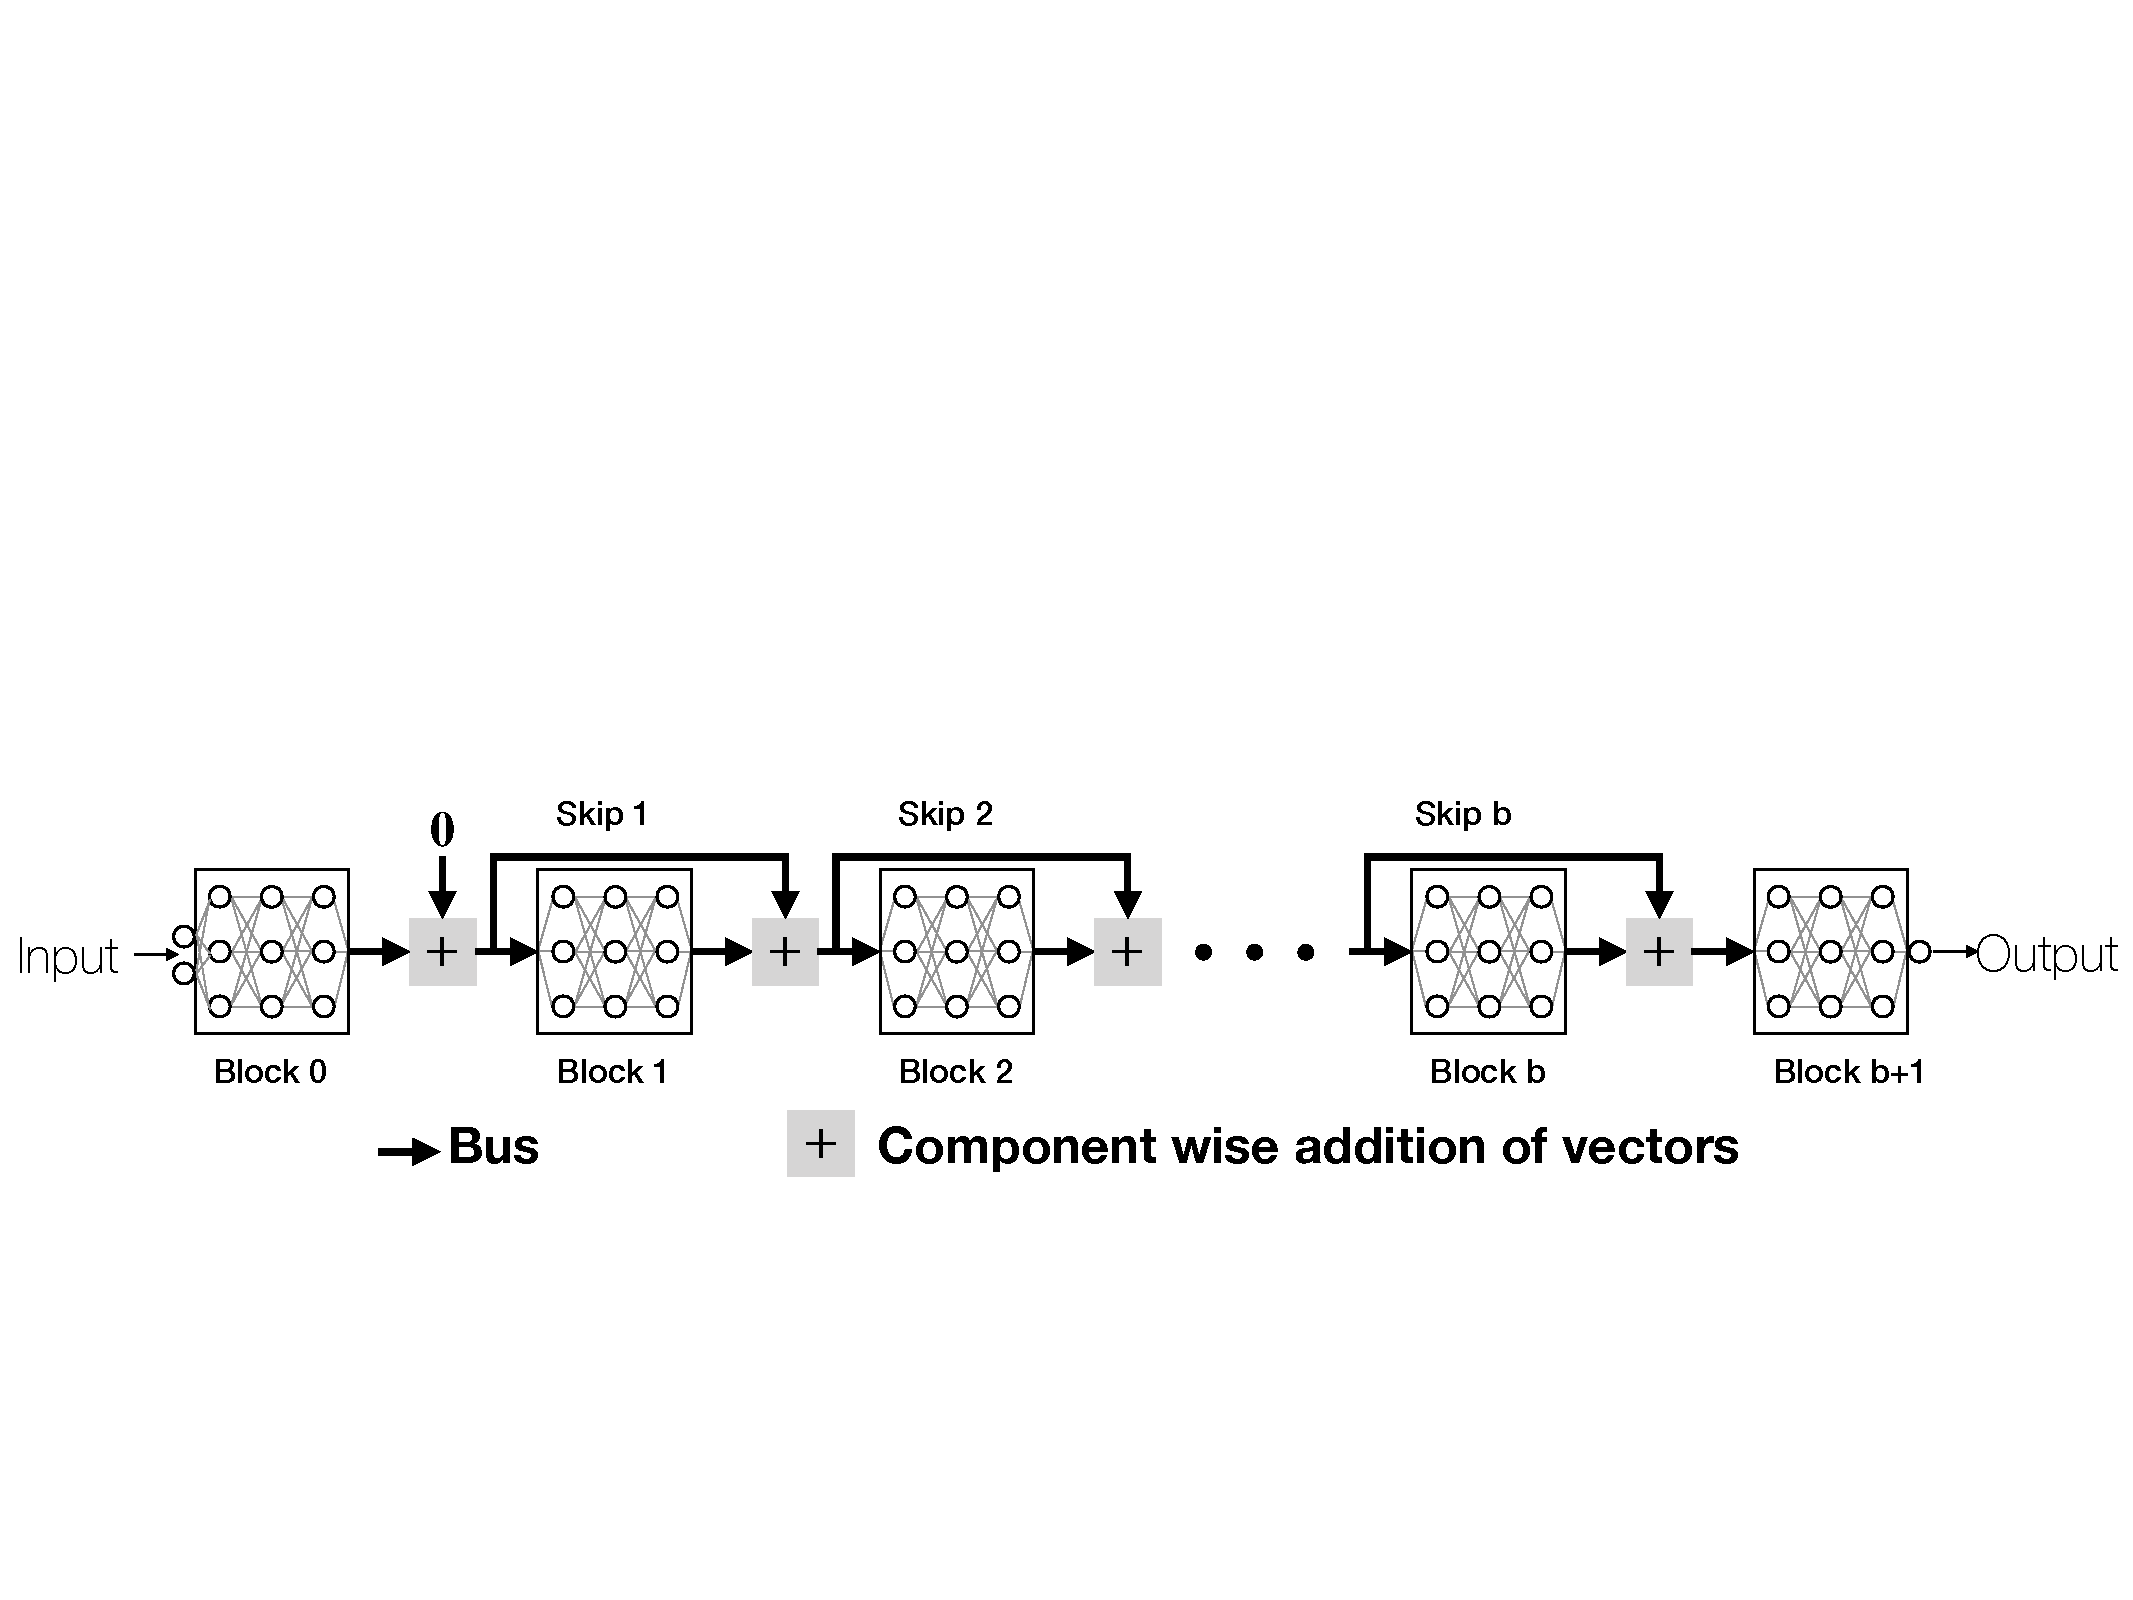
\includegraphics[scale=0.5]{figs/resnet.pdf}
}
\caption{ResNet with $b$ skip connections and $(b+2)$ blocks.}
\label{fig:resnet}
\end{figure}
\begin{definition}\label{def:subfcdnn}[Sub FC-DNNs]
Let $2^{[b]}$ denote the power set of $[b]$ and let $\J\in 2^{[b]}$ denote any subset of $[b]$. Define the`$\J^{th}$' sub-FC-DNN of the ResNet to be the fully connected network obtained by ignoring/removing (see \Cref{fig:resnet}) the skip connections $\text{skip}_j,\forall j\in \J$ (see \Cref{fig:resnet}).
\end{definition}
\Cref{fig:subfcdnn} shows the $4$ sub-FC-DNNs namely $H^i,i=1,2,3,4$ in the case of $b=2$ skip connections.
\FloatBarrier
\begin{figure}[h]
\resizebox{\columnwidth}{!}{
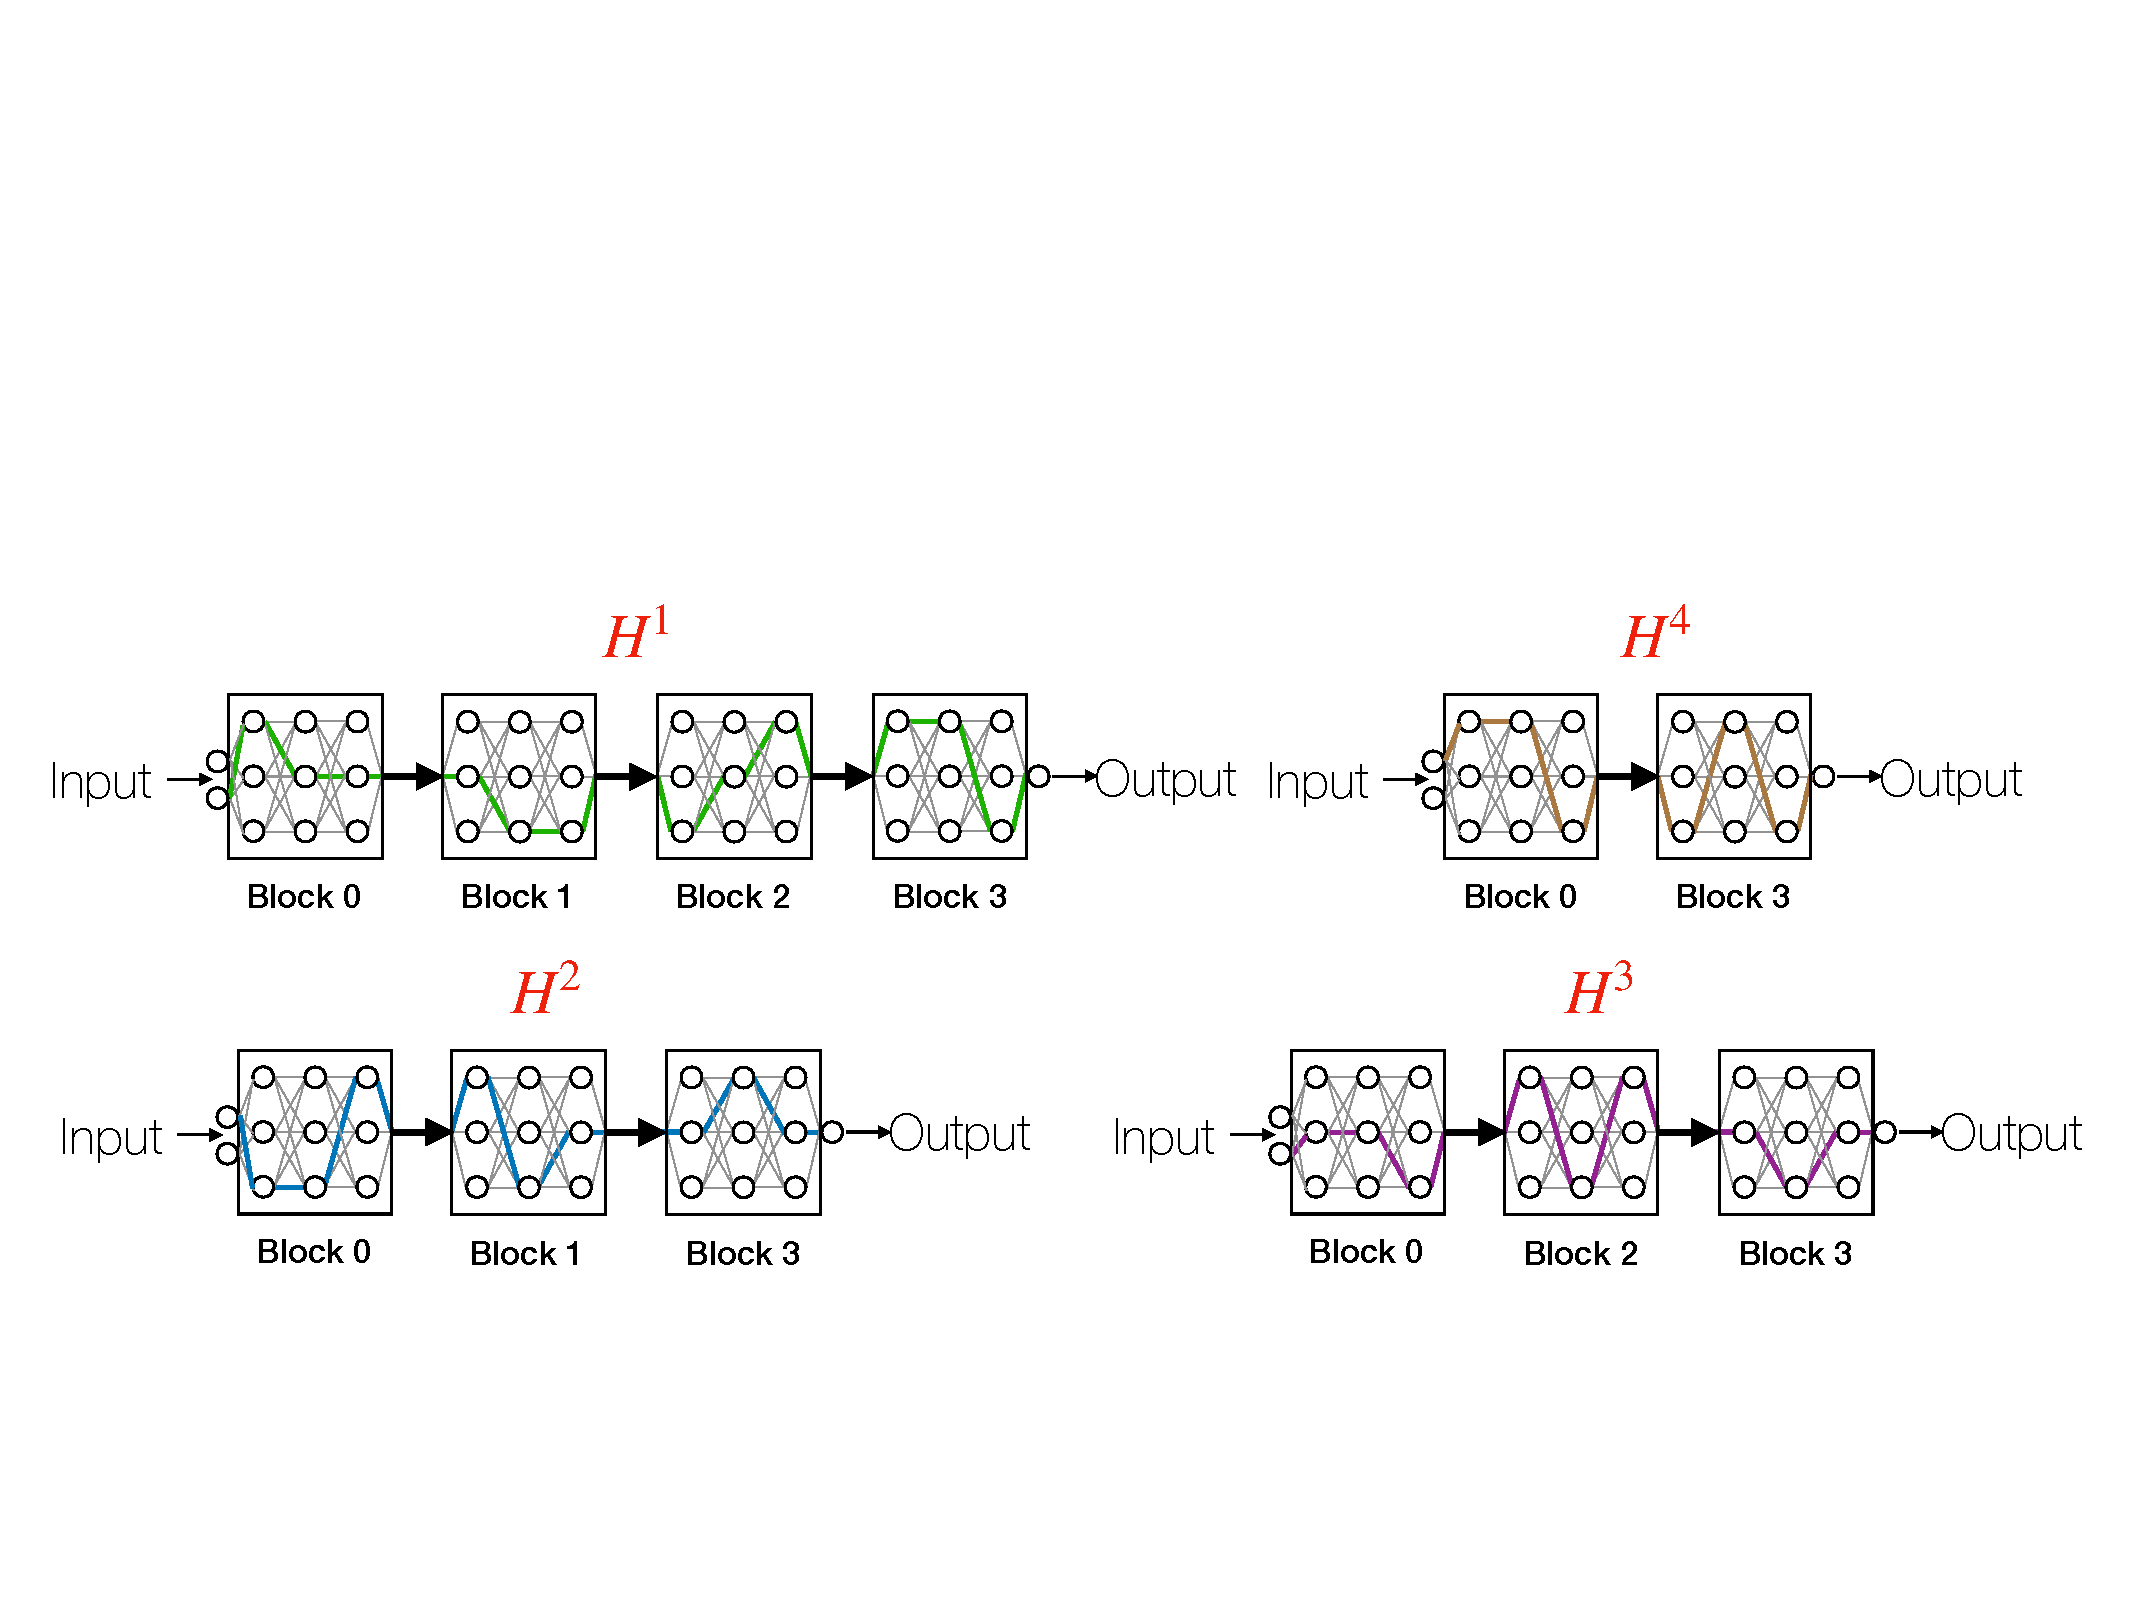
\includegraphics[scale=0.5]{figs/blocks.pdf}
}
\caption{The $2^2$ sub-FC-DNNs in a ResNet with $b=2$.}
\label{fig:subfcdnn}
\end{figure}
\begin{notation}[Index Maps]
Let $\I^{\J}(p)\colon [\Pres]\ra 2^{[b]}$ specify the indices of the skip connections ignored in path $p$.  Also, we follow the convention that weights and gating values of layers corresponding to blocks skipped are $1$.
\end{notation}

\begin{lemma}[Sum of Product Kernel]\label{lm:sumofproduct}
Let $H^{\text{res}}_{\Theta}$ be the NPK of the ResNet, and $H^{\J}_{\Theta}$ be the NPK of the sub-FC-DNN within the ResNet obtained by ignoring those skip connections in the set $\J$. Then, \begin{align*}H^{\text{res}}_{\Theta}=\sum_{\J\in 2^{[b]}}H^{\J}_{\Theta}\end{align*}
%\begin{align*}
%\end{align*}
\end{lemma}

\begin{theorem}\label{th:main} Let $\sigma=\frac{\sigfc}{\sqrt{w}}$ in \Cref{assmp:main}. As $w\ra\infty$, for ResNet we have for $\bres^{\J} = (|\J| +2)\dblock \sigfc^{2\big( (|\J|+2)\dblock-1\big)}$
\begin{align*}
\kv_{\Tdgn_0}\ra \sum_{\J\in 2^{[b]}}  \bres^{\J} H^{\J}_{\Tf_0}
\end{align*}
\end{theorem}